\let\negmedspace\undefined
\let\negthickspace\undefined
\documentclass[journal,12pt,onecolumn]{IEEEtran}
\usepackage{cite}
\usepackage{amsmath,amssymb,amsfonts,amsthm}
\usepackage{algorithmic}
\usepackage{graphicx}
\graphicspath{{./figs/}}
\usepackage{textcomp}
\usepackage{xcolor}
\usepackage{txfonts}
\usepackage{listings}
\usepackage{enumitem}
\usepackage{mathtools}
\usepackage{gensymb}
\usepackage{comment}
\usepackage{caption}
\usepackage[breaklinks=true]{hyperref}
\usepackage{tkz-euclide} 
\usepackage{listings}
\usepackage{gvv}                                        
%\def\inputGnumericTable{}                                 
\usepackage[latin1]{inputenc}     
\usepackage{xparse}
\usepackage{color}                                            
\usepackage{array}                                            
\usepackage{longtable}                                       
\usepackage{calc}                                             
\usepackage{multirow}
\usepackage{multicol}
\usepackage{hhline}                                           
\usepackage{ifthen}                                           
\usepackage{lscape}
\usepackage{tabularx}
\usepackage{array}
\usepackage{float}
%\newtheorem{theorem}{Theorem}[section]
%\newtheorem{theorem}{Theorem}[section]
%\newtheorem{problem}{Problem}
%\newtheorem{proposition}{Proposition}[section]
%\newtheorem{lemma}{Lemma}[section]
%\newtheorem{corollary}[theorem]{Corollary}
%\newtheorem{example}{Example}[section]
%\newtheorem{definition}[problem]{Definition}

\begin{document}

%\textbf{\Large 2.6.38} \\
%\textbf{\large AI25BTECH11027 - NAGA BHUVANA} \\
\title{2.6.38}
\author{AI25BTECH11027 - NAGA BHUVANA}
% \maketitle
% \newpage
% \bigskip
%\begin{document}
{\let\newpage\relax\maketitle}
%\renewcommand{\thefigure}{\theenumi}
%\renewcommand{\thetable}{\theenumi}
\noindent
		\textbf{Question:}\\
If $\vec{a}=\hat{i}+\hat{j}+\hat{k}$ and $\vec{b}=\hat{j}-\hat{k}$, find a vector $\vec{c}$ such that $\vec{a} \times \vec{c}=\vec{b}$ and $\vec{a} \cdot \vec{c}=3$\\
\textbf{Solution:}\\
	Given that
    \begin{align}
        \vec{a}=\myvec{1\\1\\1},\vec{b}=\myvec{0\\1\\-1}
    \end{align}
    
    \begin{align}
        \vec{a}^T\vec{c}=3\\
        \vec{b}^T\vec{c}=0
    \end{align}
    \begin{align}
        \myvec{\vec{a} && \vec{b}}^T\vec{c}=\myvec{3\\0}
    \end{align}
   \begin{align}
       \myvec{1&1&1\\0&1&-1}\vec{c}=\myvec{3\\0}
   \end{align}
   By solving\\
   \begin{align}
       \vec{c}=\myvec{3\\0\\0}+\lambda \myvec{-2\\1\\1}=\myvec{3-2\lambda \\ \lambda \\ \lambda}
   \end{align}
 \begin{align}
	 \lambda=\frac{2}{3} \quad \text{Satisfies the cross product condition}
   \end{align}
   \begin{align}
       \vec{c}=\myvec{\frac{5}{3}\\ \frac{2}{3}\\ \frac{2}{3}}
   \end{align}
   \begin{center}
   $\therefore$ $\vec{c}=\frac{5}{3}\hat{i}+\frac{2}{3}\hat{j}+\frac{2}{3}\hat{k}$
   \end{center}
   \begin{figure}[H]
	   \centering
	   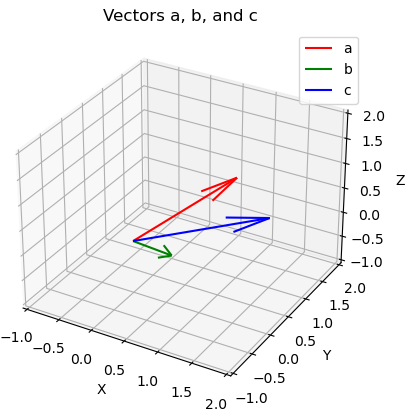
\includegraphics[width=0.7\linewidth]{figs/fig1.png}
	   \caption{}
	   \label{fig}
   \end{figure}
   \end{document}
